%\documentclass[8pt,handout]{beamer}
\documentclass[8pt]{beamer}

%-----------------------------------------------------------------
%	Packages
%-----------------------------------------------------------------
\usepackage{animate}
\usepackage[utf8]{inputenc}	% für Umlaute ect.
\usepackage{fancyhdr} % für header
\usepackage{lastpage} % für footer
\usepackage{extramarks} % für header und footer
\usepackage{amsthm} % math stuff
\usepackage{amsmath} % math stuff
\usepackage{amssymb} % math stuff
\usepackage{color}
\usepackage{listings} % code listings
\usepackage{graphicx} % für graphics
\usepackage{color}
\usepackage{tikz}
\usepackage[absolute,overlay]{textpos} %to translate graphics through space
\usepackage{soul}
\usepackage{hyperref}
\usepackage{xcolor}
\usepackage{textpos}


\newcommand{\highlightred}[1]{%
	\colorbox{red!50}{$\displaystyle#1$}}
\newcommand{\highlightgreen}[1]{%
	\colorbox{green!50}{$\displaystyle#1$}}
\newcommand{\highlightblue}[1]{%
	\colorbox{blue!50}{$\displaystyle#1$}}
\newcommand{\highlightyellow}[1]{%
	\colorbox{yellow!50}{$\displaystyle#1$}}


%-----------------------------------------------------------------
%	Title
%-----------------------------------------------------------------
\title{ABS-Normal Form}
\subtitle{Eine Implementierung mit CUDA}
\author[Matthias Mitterreiter]{
\includegraphics[height=3cm,width=4cm]{img/badge-nvidia-cuda-cpp}  \\ Matthias Mitterreiter}
\institute{Seminar Parallel Computing - FSU Jena \\
%\vspace{0.5cm}
{\scriptsize Prof. Martin Bücker, Dr. Torsten Bosse, Dipl-Inf. Ralf Seidler}}
\date{\today}

%-----------------------------------------------------------------
%	Settings
%-----------------------------------------------------------------


\mode<presentation>
{
	\usetheme{Warsaw}
	\usecolortheme{crane}
}


%---------------------------------------------------
%	Colors
%---------------------------------------------------

\definecolor{listing-background}{RGB}{77,77,77}
\definecolor{manifest-green}{RGB}{0, 179, 0}
\definecolor{orange}{RGB}{255,127,0}
\definecolor{green}{RGB}{57, 230, 0}
\definecolor{blue}{RGB}{26, 117, 255}
\definecolor{yellow}{RGB}{254, 255, 102}
\definecolor{red}{RGB}{255,77,77}
\definecolor{blue2}{RGB}{51, 204, 255}
\definecolor{lightgray}{rgb}{.9,.9,.9}
\definecolor{darkgray}{rgb}{.4,.4,.4}
\definecolor{purple}{rgb}{0.65, 0.12, 0.82}

%---------------------------------------------------
%	Syntax Highlighting
%---------------------------------------------------

\lstdefinelanguage{manifest}{
  keywords={CACHE, NETWORK, FALLBACK,MANIFEST},
  morecomment=[s]{/*}{*/},
  morecomment=[l]{\#}, 
  morestring=[b]',
  morestring=[b]",
  ndkeywords={class, export, boolean, throw, implements, import, this},
  keywordstyle=\color{manifest-green}\bfseries,
  ndkeywordstyle=\color{black}\bfseries,
  identifierstyle=\color{black},
  commentstyle=\color{purple}\ttfamily,
  stringstyle=\color{red}\ttfamily,
  sensitive=true
}

\lstdefinelanguage{JavaScript}{
  keywords={CACHE, NETWORK, FALLBACK,MANIFEST, break, case, catch, continue, debugger, default, delete, do, else, false, finally, for, function, if, in, instanceof, new, null, return, switch, this, throw, true, try, typeof, var, void, while, with},
  morecomment=[l]{//},
  morecomment=[s]{/*}{*/},
  morestring=[b]',
  morestring=[b]",
  ndkeywords={class, export, boolean, throw, implements, import, this},
  keywordstyle=\color{blue}\bfseries,
  ndkeywordstyle=\color{darkgray}\bfseries,
  identifierstyle=\color{black},
  commentstyle=\color{purple}\ttfamily,
  stringstyle=\color{red}\ttfamily,
  sensitive=true
}
\lstdefinelanguage{cuda}{
	keywords={cudaMemcpy, cudaMemcpyDeviceToDevice},
	morecomment=[l]{//},
	morecomment=[s]{/*}{*/},
	morestring=[b]',
	morestring=[b]",
	ndkeywords={class, if, while, boolean, for, int, bool, double, ffloat, template, typename},
	keywordstyle=\color{blue}\bfseries,
	ndkeywordstyle=\color{darkgray}\bfseries,
	identifierstyle=\color{black},
	commentstyle=\color{purple}\ttfamily,
	stringstyle=\color{red}\ttfamily,
	sensitive=true
}
\definecolor{dkgreen}{rgb}{0,0.6,0}
\definecolor{dred}{rgb}{0.545,0,0}
\definecolor{dblue}{rgb}{0,0,0.545}
\definecolor{lgrey}{rgb}{0.9,0.9,0.9}
\definecolor{gray}{rgb}{0.4,0.4,0.4}
\definecolor{darkblue}{rgb}{0.0,0.0,0.6}
\lstdefinelanguage{cpp}{
	backgroundcolor=\color{lgrey},  
	basicstyle=\footnotesize \ttfamily \color{black} \bfseries,   
	breakatwhitespace=false,       
	breaklines=true,               
	captionpos=b,                   
	commentstyle=\color{dkgreen},   
	deletekeywords={...},          
	escapeinside={\%*}{*)},                  
	frame=single,                  
	language=C++,                
	keywordstyle=\color{purple},  
	morekeywords={BRIEFDescriptorConfig,string,TiXmlNode,DetectorDescriptorConfigContainer,istringstream,cerr,exit},
	ndkeywords={cudaMemcpy, cudaMemcpyDeviceToDevice, cublasDgemv},
	ndkeywordstyle=\color{blue},
	identifierstyle=\color{black},
	stringstyle=\color{blue},      
	numbers=left,                 
	numbersep=5pt,                  
	numberstyle=\tiny\color{black}, 
	rulecolor=\color{black},        
	showspaces=false,               
	showstringspaces=false,        
	showtabs=false,                
	stepnumber=1,                   
	tabsize=2,                     
	title=\lstname,                 
}
%\lstset{
%   language=JavaScript,
%   backgroundcolor=\color{lightgray},
%   extendedchars=true,
%   basicstyle=\footnotesize\ttfamily,
%   showstringspaces=false,
%   showspaces=false,
%   numbers=left,
%   numberstyle=\footnotesize,
%   numbersep=7pt,
%   tabsize=2,
%   breaklines=true,
%   showtabs=false,
%   captionpos=b,
%   literate={\ \ }{{\ }}1
%}

\definecolor{mygray}{rgb}{0.4,0.4,0.4}
\definecolor{mygreen}{rgb}{0,0.8,0.6}
\definecolor{myorange}{rgb}{1.0,0.4,0}

\lstset{
	basicstyle=\footnotesize\sffamily\color{black},
	commentstyle=\color{mygray},
	frame=single,
	numbers=left,
	numbersep=5pt,
	numberstyle=\tiny\color{mygray},
	keywordstyle=\color{mygreen},
	showspaces=false,
	showstringspaces=false,
	stringstyle=\color{myorange},
	tabsize=2
}

% An environment for stpes, cases ect. 
% From: http://tex.stackexchange.com/questions/32798/a-step-by-step-environment
\newenvironment{steps}[1]{\begin{enumerate}[label=#1 \arabic*]}{\end{enumerate}}
\makeatletter%
\def\step{%
	\@ifnextchar[ \@step{\@noitemargtrue\@step[\@itemlabel]}}
\def\@step[#1]{\item[#1]\mbox{}\\\hspace*{\dimexpr-\labelwidth-\labelsep}}
\makeatother

%-----------------------------------------------------------------------------
%	Theoreme
%-----------------------------------------------------------------------------
\newtheorem{mydef}{Definition}
\newtheorem*{mydef*}{Definition}
\newtheorem{mybei}{Beispiel}
\newtheorem*{mybei*}{Beispiel}\usepackage{tikz}
\newtheorem{mysatz}{Satz}
\newtheorem*{mysatz*}{Satz}
\newtheorem{mybew}{Beweis}
\newtheorem*{mybew*}{Beweis}
\newtheorem{myfolg}{Folgerung}
\newtheorem*{myfolg*}{Folgerung}
\newtheorem{mybemerk}{Bemerkung}
\newtheorem*{mybemerk*}{Bemerkung}


%-------------------------------------------------
%	Beamer
%-------------------------------------------------
%\definecolor{craneorange}{rgb}{0.68,1,1}
%\definecolor{craneblue}{gray}{0.85}

\newcommand\x{\times}

% requires version 0.3 of the package
\usepackage[customcolors]{hf-tikz}

\tikzset{style green/.style={
		set fill color=green!50!lime!60,
		set border color=white,
	},
	style cyan/.style={
		set fill color=cyan!90!blue!60,
		set border color=white,
	},
	style orange/.style={
		set fill color=orange!80!red!60,
		set border color=white,
	},
	hor/.style={
		above left offset={-0.15,0.31},
		below right offset={0.15,-0.125},
		#1
	},
	ver/.style={
		above left offset={-0.1,0.3},
		below right offset={0.15,-0.15},
		#1
	}
}
\begin{document}

\maketitle

\addtobeamertemplate{frametitle}{}{%
\begin{tikzpicture}[remember picture,overlay]
\node[anchor=north east,yshift=1pt] at (current page.north east) {
\includegraphics[height=0.8cm]{img/badge-nvidia-cuda-cpp}};
\end{tikzpicture}}
	\begin{frame}
\frametitle{Inhalt}
\framesubtitle{...}
	\begin{enumerate}
		\item ABS - Normal Form
		\item Aufgabengeschreibung
		\item Implementierung
		\begin{enumerate}
			\item Verwendete Bibliotheken
			\item Evaluate
			\item Gradient
			\item Solve
		\end{enumerate}
		\item Anwendung
		\item Numerische Tests und Vergleiche
		\item Cool Snippets
		\item Imprevements
		\item Problems Lesson Learned
	\end{enumerate}
\end{frame}
%------------------------------------------------------------------------
\begin{frame}
	\frametitle{ABS-NF}
	\framesubtitle{Einführung}
	\setbeamertemplate{enumerate items}[default]
	\begin{mydef*}
		Smooth funcion \\
		A smooth function $f(x)$ is continuous and has a continuous derivative
	\end{mydef*}
	$f(x) = x^2$ $f'(x) = 2x$

\end{frame}
%------------------------------------------------------------------------
\begin{frame}
	\frametitle{ABS-NF}
	\framesubtitle{Einführung}
	\setbeamertemplate{enumerate items}[default]
	\begin{mydef*}
		Picewise smooth function \\
		A picewise smooth function $f(x)$ is made up of finitly many smooth functions, separated by
		jump discontiuities.
	\end{mydef*}
	\begin{flalign*}
		f(x) = \begin{cases}
			1 & x < -1 \\
			x^2 + 1 & -1 <= x < 2 \\
			x & 2 <= x
		\end{cases}
	\end{flalign*}
	Wir betrachten ausschließlich continuous picewise smooth functions.
\end{frame}
%------------------------------------------------------------------------
\begin{frame}
\frametitle{ABS-NF}
\framesubtitle{Einführung}
	Picewise smooth  funcitons können durch picewise linear functions (PL) approximiert werden.
	\begin{center}
		BILD
	\end{center}
	Betrachten ausschließlich continuous PL
\end{frame}
%------------------------------------------------------------------------
\begin{frame}
	\frametitle{ABS-NF}
	\framesubtitle{Einführung}
	\setbeamertemplate{enumerate items}[default]
	ABS-Normal Form:
	\begin{center}
		Repräsentierung für Picewise linear functions (PL) 
	\end{center}
	\begin{flalign*}
	\begin{pmatrix}
	\Delta z \\
	\Delta y
	\end{pmatrix}
	= 
	\begin{pmatrix}
	a \\
	b
	\end{pmatrix}
	+
	\begin{pmatrix}
	Z & L \\
	J & Y 
	\end{pmatrix}
	\times
	\begin{pmatrix}
	\Delta x \\
	|\Delta z |
	\end{pmatrix}
	\end{flalign*}
\end{frame}
%------------------------------------------------------------------------
\begin{frame}
	\frametitle{ABS-NF}
	\framesubtitle{Einführung}
	\setbeamertemplate{enumerate items}[default]
	Vorgehen:
	\begin{itemize}
		\item Any picewise linear scalar function has a so called min-max repräsentation
		\item All min max expressions can be expressed in terms of abs functions
		\item Picewise linearization wird erreicht durch algorithmic differentiation
	\end{itemize}
\end{frame}
%------------------------------------------------------------------------
\begin{frame}
	\frametitle{ABS-NF}
	\framesubtitle{Beispiel}
	\setbeamertemplate{enumerate items}[default]
	\begin{flalign*}
		F(x_1,x_2) &= (x_2^2 - x_1^+)^+ \\
			 (i)^+ &= \max(0, i)
	\end{flalign*}
	\begin{center}
		BILD
	\end{center}
	
\end{frame}
%------------------------------------------------------------------------
\begin{frame}
	\frametitle{ABS-NF}
	\framesubtitle{Einführung}
	\setbeamertemplate{enumerate items}[default]
	\begin{center}
		ADOL C, Beispiel
	\end{center}
\end{frame}
%------------------------------------------------------------------------
\begin{frame}
	\frametitle{ABS-NF}
	\framesubtitle{Aufgabenbeschreibung}
	\setbeamertemplate{enumerate items}[default]
	\begin{itemize}
		\item Evaluate abs normal form
		\item Calculate Gradient
		\item Solve abs-normal form system
	\end{itemize}
\end{frame}
%------------------------------------------------------------------------
	%------------------------------------------------------------------------
\begin{frame}
	\frametitle{Content}
	\framesubtitle{ABS-Normal Form}
	\begin{columns}[T] % align columns
		\begin{column}{.48\textwidth}
			
			\begin{center}
				{\Huge Aufgaben}
			\end{center}
			
		\end{column}%
		\hfill%
		\begin{column}{.48\textwidth}
			\color{blue}\rule{\linewidth}{4pt}
			
			\setbeamertemplate{enumerate items}[default]
			\begin{enumerate}
				\item Einführung
				\item \textbf{Aufgaben}
				\item Evaluate
				\item Gradient
				\item Blocksize und Gridsize
				\item Solve
				\item Final Thoughts
			\end{enumerate}
		\end{column}%
	\end{columns}
\end{frame}
%------------------------------------------------------------------------
\begin{frame}
	\frametitle{ABS-NF}
	\framesubtitle{Aufgabenbeschreibung}
	\setbeamertemplate{enumerate items}[default]
	\begin{flalign*}
	\begin{pmatrix}
	\Delta z \\
	\Delta y
	\end{pmatrix}
	= 
	\begin{pmatrix}
	a \\
	b
	\end{pmatrix}
	+
	\begin{pmatrix}
	Z & L \\
	J & Y 
	\end{pmatrix}
	\times
	\begin{pmatrix}
	\Delta x \\
	|\Delta z |
	\end{pmatrix}
	\end{flalign*}
	Aufgaben:
	\begin{itemize}
		\item <1-> Evaluate abs normal form:
			\begin{itemize}
				\item Geg: $a,b,Z,L,J,Y,\Delta x$
				\item Ges: $\Delta z, \Delta y$
			\end{itemize}
		\item <2-> Calculate Gradient
			\begin{itemize}
				\item Geg: $a,b,Z,L,J,Y, \Delta Z$
				\item Ges: Gradient $\gamma, \Gamma$
			\end{itemize}
		\item <3-> Solve abs-normal form
		\begin{itemize}
			\item Geg: $a,b,Z,L,J,Y,\Delta y$
			\item Ges: $\Delta x, \Delta Z$
		\end{itemize}
	\end{itemize}
\end{frame}
%------------------------------------------------------------------------
\begin{frame}
	\frametitle{ABS-NF}
	\framesubtitle{Annahmen und Voraussetzung und Info zur Implementierung}
	\setbeamertemplate{enumerate items}[default]
	Programmiersprachen
	\begin{itemize}
		\item Python 3.5: Prototyping und Serial Performance benchmarks
		\item Cuda C++: Implementierung der paralleln ABS-NF Aufgaben
	\end{itemize}
	
	Annahmen:
	\begin{enumerate}
		\item Global memory der GPU ist groß genug um alle benötigten Datenstrukturen zeitgleich zu halten
		\item Daten werden vektorisiert übergeben
		\item Sofern möglich mappe alle Problem auf existierende Librariers
	\end{enumerate}
	
\end{frame}
%------------------------------------------------------------------------
\begin{frame}[fragile]
	\frametitle{ABS-NF}
	\framesubtitle{Implementierung}
	\setbeamertemplate{enumerate items}[default]
	Benutzte Libraries:
	\begin{itemize}
		\item cuBLAS (cuda Basic Linear Algebra Subprograms)
		\begin{itemize}
			\item Matrix Vector operations
			\item Matrix Matrix operations
		\end{itemize}
		\item cuSOLVER
		\begin{itemize}
			\item Matrix factorization
			\item Triangular solve
		\end{itemize}
		\item C++ STL
	\end{itemize}
\begin{lstlisting}[language=C++]
#include <cublas_v2.h>
#include <cusolverDn.h>
\end{lstlisting}

\begin{lstlisting}
	nvcc -std=c++11 x.cu -lcublas -lcusolver -o x
\end{lstlisting}
	
\end{frame}
%------------------------------------------------------------------------
	%------------------------------------------------------------------------
\begin{frame}
	\frametitle{Content}
	\framesubtitle{ABS-Normal Form}
	\begin{columns}[T] % align columns
		\begin{column}{.48\textwidth}
			
			\begin{center}
				{\Huge Evaluate}
			\end{center}
			
		\end{column}%
		\hfill%
		\begin{column}{.48\textwidth}
			\color{blue}\rule{\linewidth}{4pt}
			
			\setbeamertemplate{enumerate items}[default]
			\begin{enumerate}
				\item Einführung
				\item Aufgaben
				\item \textbf{Evaluate}
				\item Gradient
				\item Blocksize und Gridsize
				\item Solve
				\item Final Thoughts
			\end{enumerate}
		\end{column}%
	\end{columns}
\end{frame}
%------------------------------------------------------------------------
\begin{frame}
	\frametitle{Aufgabe 1) Evaluate}
	\framesubtitle{Aufgabenstellung und Problem}
	\setbeamertemplate{enumerate items}[default]
	ABS-Normal Form:
	\begin{flalign*}
		\begin{pmatrix}
		\Delta z \\
		\Delta y
		\end{pmatrix}
		= 
		\begin{pmatrix}
		a \\
		b
		\end{pmatrix}
		+
		\begin{pmatrix}
		Z & L \\
		J & Y 
		\end{pmatrix}
		\times
		\begin{pmatrix}
		\Delta x \\
		|\Delta z |
		\end{pmatrix}
	\end{flalign*}
	Gegeben:
	\begin{flalign*}
		a,b,Z,L,J,Y,m,n,s, \Delta x
	\end{flalign*}
	Gesucht:
	\begin{flalign*}
		\Delta z, \Delta y
	\end{flalign*}
	\pause
	\begin{flalign*}
		\Delta y &= b + (J \times \Delta x) + (Y \times |\Delta z|) \\
		\Delta z &= a + (J \times \Delta x) + (L \times |\Delta z|)
	\end{flalign*}
	\pause
	Problem:
	\begin{flalign*}
		\highlightred{\Delta z} &= a + (J \times \Delta x) + (L \times\highlightred{ |\Delta z|})
	\end{flalign*}
\end{frame}
%----------------------------------------------------------------------------
\begin{frame}
\frametitle{Aufgabe 1) Evaluate}
\framesubtitle{Löse $z = f(|\Delta z|)$}
\setbeamertemplate{enumerate items}[default]

	
\begin{flalign*}
	\left(\begin{array}{c}
	\Delta z_1 \\
	\Delta z_2 \\
	\Delta z_3 \\
	\Delta z_4 \\
	\end{array}\right) = 
	\left(\begin{array}{c}
	k_1 \\
	k_2 \\
	k_3 \\
	k_4 \\
	\end{array}\right) +
	\left(\begin{array}{cccc}
	0 		& 0 	  & 0  & 0 \\
	L_{2,1} & 0 	  & 0  & 0 \\
	L_{3,1} & L_{3,2} & 0  & 0\\
	L_{4,1} & L_{4,2} & L_{4,3} & 0 \\
	\end{array}\right) \times
	\left(\begin{array}{c}
	|\Delta z_1 | \\
	|\Delta z_2 | \\
	|\Delta z_3 | \\
	|\Delta z_4 | \\
	\end{array}\right)
\end{flalign*}
\begin{flalign*}
	k = a + Z \times \Delta x
\end{flalign*}

\begin{flalign*}
	\onslide<1-> {\highlightblue{\Delta  z_1}  &= \underbrace{L_1 \times |\Delta z|}_{=0} + k_1 = k_1} \\
	\pause
	\onslide<2->{\highlightyellow{\Delta z_2} &= L_2 \times |\Delta z| + k_2 \\
								 &= L_{2,1} \times \highlightblue{|\Delta z_1 |} + k_2 \\}
		\onslide<3->{\highlightgreen{\Delta z_3} &= L_3 \times |\Delta z| + k_3 \\
		&= L_{3,1} \times \highlightblue{|\Delta z_1 |} + L_{3,2} \times \highlightyellow{|\Delta z_2|} + k_3 \\}
		\onslide<4->{\highlightred{\Delta z_4} &= L_{4} \times |\Delta z| + k_4 \\
		&= L_{4,1} \times \highlightblue{|\Delta z_1|} + 
		L_{4,2} \times \highlightyellow{|\Delta z_2|} +
		L_{4,3} \times \highlightgreen{|\Delta z_3|} + k_4 \\}
\end{flalign*}
\end{frame}
%----------------------------------------------------------------------------
\begin{frame}[fragile]
	\frametitle{Aufgabe 1) Evaluate}
	\framesubtitle{Implementierung}
	\begin{lstlisting}[language=cpp]
	template <typename T>
	void eval(T *a, T *b, 
			  T *Z, T *L, 
			  T *J, T *Y,
			  T *dx,
			  int m, int n, int s,
			  T *dz, T *dy,
			  T *abs_dz)
	{
			// dz = a
			cudaMemcpy(dz, a, ., cudaMemcpyDeviceToDevice));
			// dz = Z * dx + dx
			cublasDgemv(.,Z, ., dx, . dz, .)
			// dz[i] = L[i]_i * |dz|_i
			for(int i=0; i<s; i++)
			{
				cublasDgemv( . ,&L[i * s], . ,abs_dz, . , &dz[i],.);
				abs <<<1,1>>>(&dz[i], &abs_dz[i], 1);
			}
			// dy = b
			cudaMemcpy(dy, b, ., cudaMemcpyDeviceToDevice);
			// dy = dy + J*dx
			cublasDgemv(.,J, ., dx, ., dy, .));
			// dy = dy + Y * |dz|
			cublasDgemv(., Y, ., abs_dz, ., dy, .));
	}
	\end{lstlisting}
\end{frame}
%----------------------------------------------------------------------------
\begin{frame}
	\frametitle{Aufgabe 1) Evaluate}
	\framesubtitle{Speicherkomplexität}
	\setbeamertemplate{enumerate items}[default]
	Speicherkomplexität: \\
	\begin{center}
		\begin{tabular}{ c | c | c | c | c | c | c | c | c | c }
		$a$ & $b$ & $Z$ & $L$ & $J$ & $Y$ & $\Delta y$ & $\Delta x$ & $\Delta z$ & $|\Delta z|$\\
		\hline
		$s$ & $m$ & $s*n$ & $s*s$ & $m*n$ & $m*s$ & $m$ & $n$ & $s$& $s$\\
		\end{tabular}
	\end{center}
	\begin{flalign*}
		(s^2 + (3 + m + n)*s + (m + 2)m + n) * sizeof(T)
	\end{flalign*}
	\pause
	Seien 
	\begin{itemize}
		\item $m = 1000, n = 1000, s=1000$
		\item Datatype: $double \approx 8 bytes$
		\item $32.048.000$ Bytes $\approx 0.032048 GB$
	\end{itemize}
	\pause
	Seien 
	\begin{itemize}
		\item $m = 1000, n = 1000, s=100.000$
		\item Datatype: $double \approx 8 bytes$
		\item $81.610.424.000$ Bytes $\approx 81.610 GB$
		\end{itemize}
\end{frame}
%----------------------------------------------------------------------------
\begin{frame}
	\frametitle{Aufgabe 1) Evaluate}
	\framesubtitle{Komplexität}
	\setbeamertemplate{enumerate items}[default]
	Komplexität:
	\begin{center}
	\begin{tabular}{ l | c | c}
		Funktion & Komplexität Seriell & Komplexität Parallel \\
		\hline
		$cudaMemcpy(dz,a)$	& $s$ & $s/p$  \\
		$cublasDgemv(Z,dx,dz)$& $s*n$ & $(s*n)/p$ \\
		$cublasDgemv(L, |dz|)$& $s*s$ & $(s*s)/p$ \\
		$cublasMemcpy(dy,b)$  & $m$  & $m/p$ \\
		$cublasDgemv(J,dx,dy)$& $m*n$ & $(m*n)/p$ \\
		$cublasDgemv(Y, |dz|, dy)$ & $m*s$ & $(m*s)/p$ \\
	\end{tabular} 	\\~\\
	\end{center}
	\pause
	Der Rechenaufwand steigt im selben Maße wie der Speicheraufwand ! \\
	\pause
	\begin{center}
		Vermutung, parallelisieren bringt hier nicht viel!
	\end{center}
\end{frame}
%----------------------------------------------------------------------------
\setbeamertemplate{navigation symbols}{}
\begin{frame}[plain]
	\makebox[\linewidth]{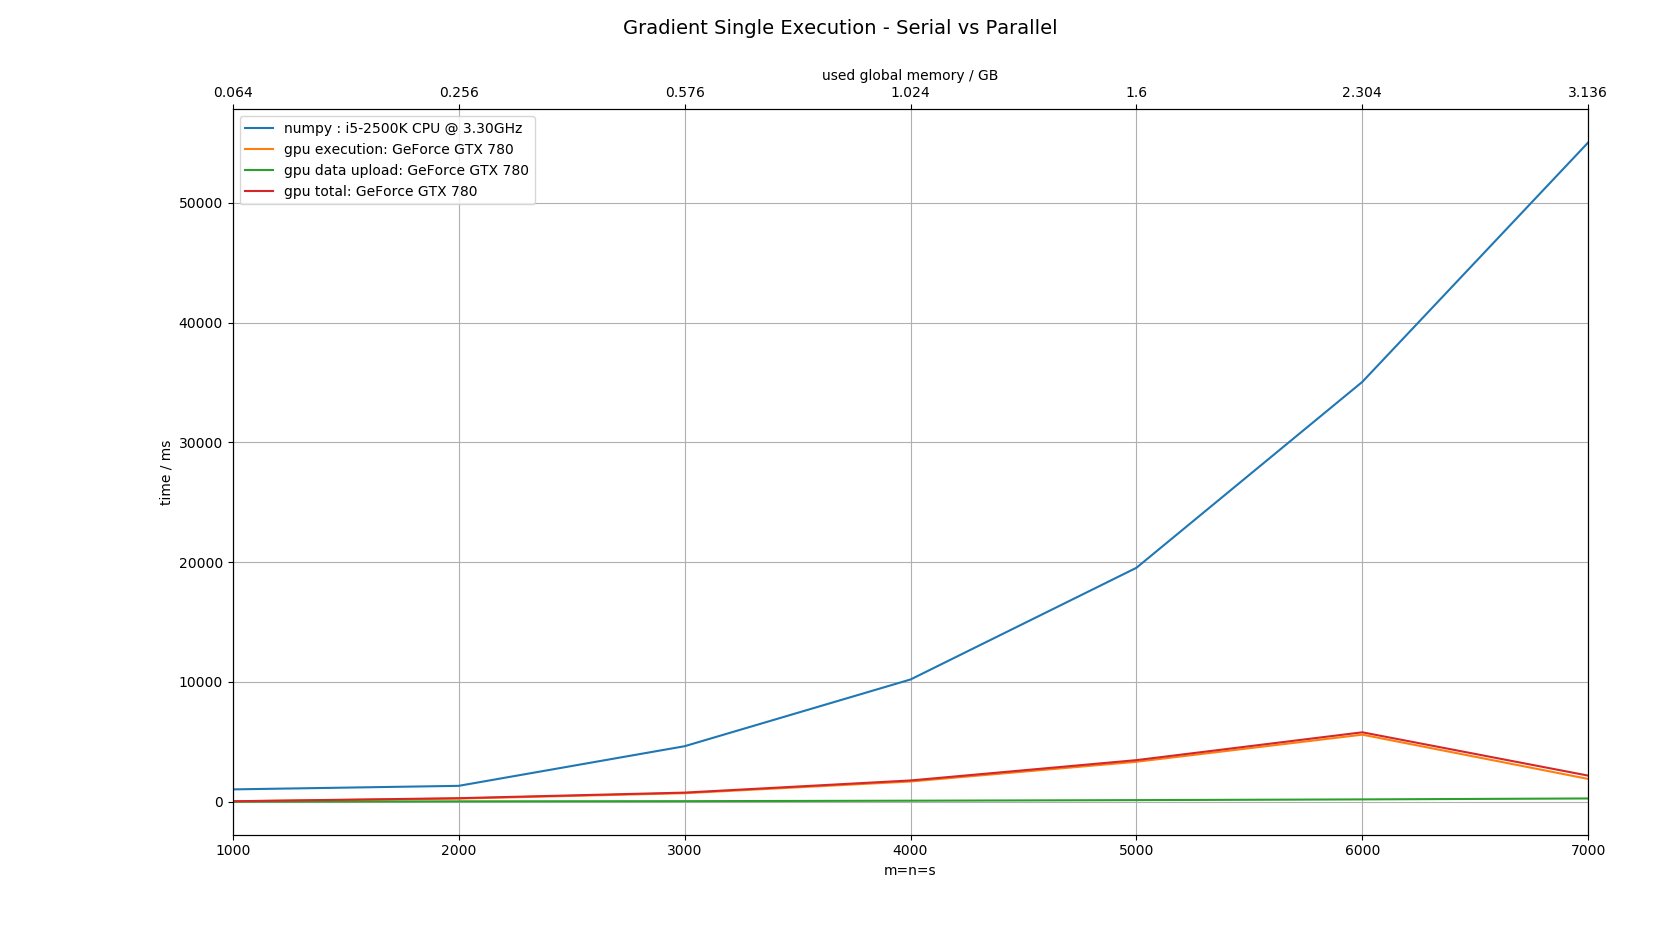
\includegraphics[width=\paperwidth]{img/eval-single.png}}
\end{frame}
%----------------------------------------------------------------------------
\setbeamertemplate{navigation symbols}{}
\begin{frame}[plain]
	\makebox[\linewidth]{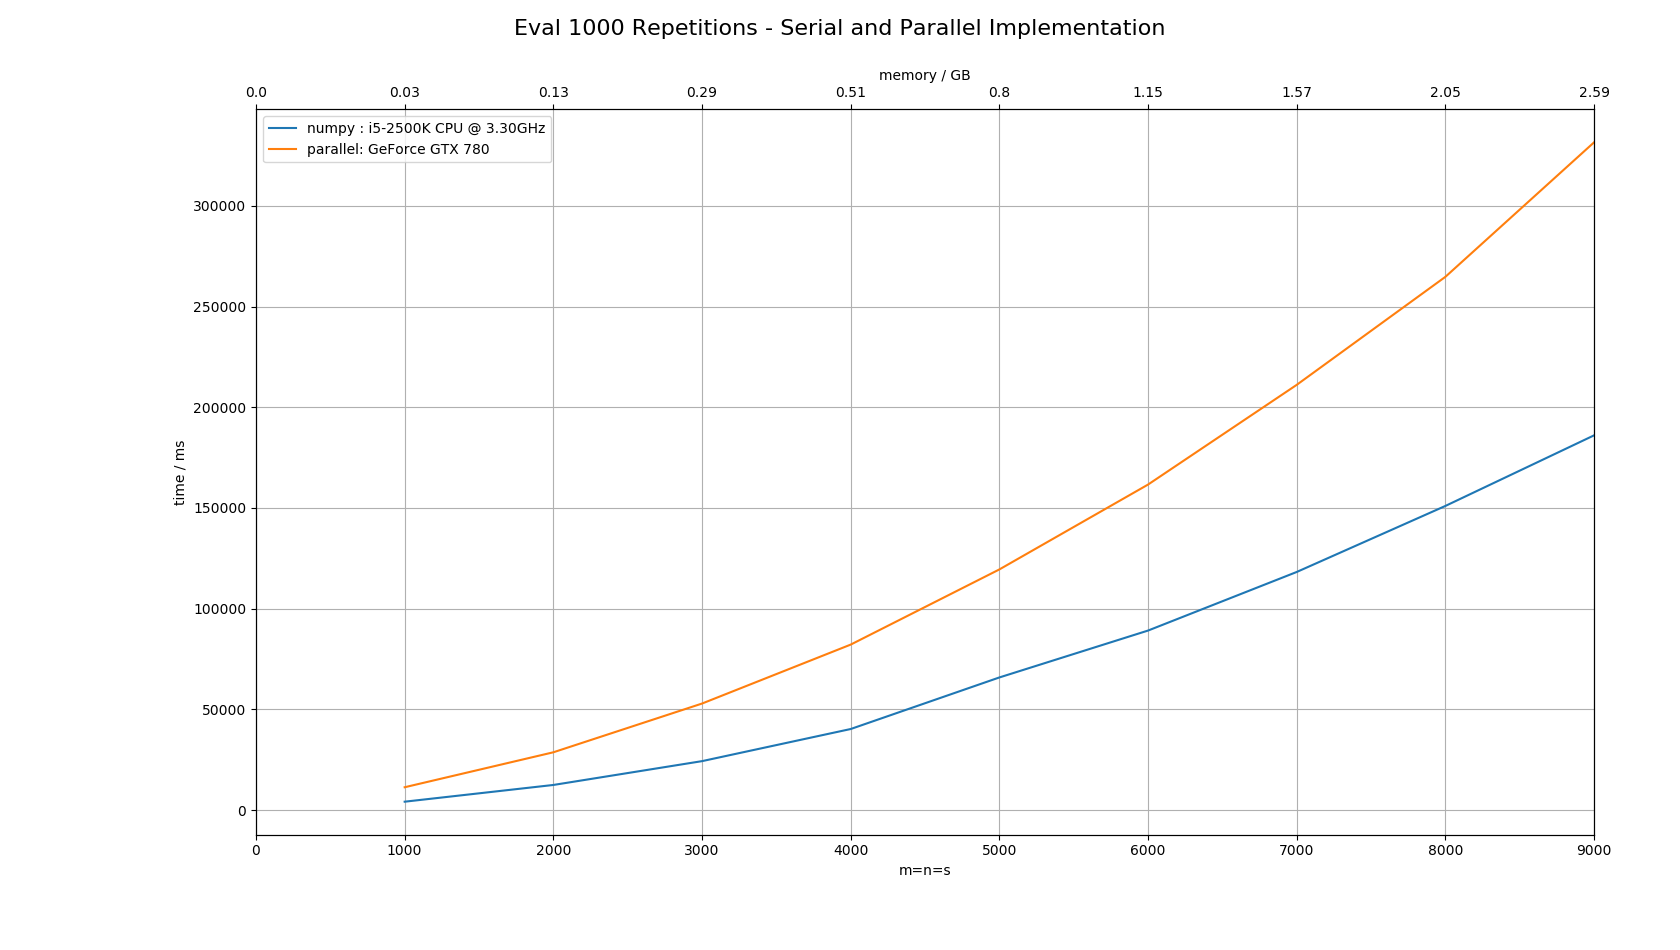
\includegraphics[width=\paperwidth]{img/eval-100.png}}
\end{frame}
	\section{Gradient}
\subsection{Problem Specification}

ABS-Normal Form:
\begin{flalign*}
\begin{pmatrix}
\Delta z \\
\Delta y
\end{pmatrix}
= 
\begin{pmatrix}
a \\
b
\end{pmatrix}
+
\begin{pmatrix}
Z & L \\
J & Y 
\end{pmatrix}
\circ
\begin{pmatrix}
\Delta x \\
|\Delta z |
\end{pmatrix}
\end{flalign*}

The problem here is to calculate the gradient of a PL function in abs-normal form. Given the following structures:
\begin{flalign*}
	a,b,Z,L,J,Y,m,n,s,\Delta z
\end{flalign*}
the gradient can be obtained in the following way:
\begin{flalign*}
	\Sigma = diag(sign(\Delta z))
\end{flalign*}
\begin{flalign*}
	\Delta z &= a + Z \Delta x + L \Sigma \Delta z \\
		     &= (I-L\Sigma)^{-1} (a+Z \Delta x) \\
	\Delta y &= b + J \Delta x + Y |\Delta z| \\
		     &= b + J \Delta x + Y \Sigma \big( (I-L\Sigma)^{-1} (a+Z \Delta x) \big) \\
		     &= b + Y \Sigma(I-L \Sigma)^{-1} a + \big( J + Y\Sigma(I-L\Sigma)^{-1}Z  \Big) \Delta x
\end{flalign*}
\begin{flalign}
	\gamma &= b + Y \Sigma(I-L \Sigma)^{-1} a \label{eq_gamma} \\
	\Gamma &= J + Y\Sigma(I-L\Sigma)^{-1}Z \label{eq_Gamma}
\end{flalign}
The gradient can now e calculated as:
\begin{flalign*}
	\Delta f(\Delta x) = \gamma + \Gamma \Delta x
\end{flalign*}

The problem task is to implement a function that calculates $\gamma$ as well as $\Gamma$.

\subsection{Implementation}

\begin{lstlisting}[language=cpp]
template <typename T>
void gradient(T *a, T *b, 
T *Z, T *L, 
T *J, T *Y,
T *dz,
T *Tss, T *I, T *K,
int m, int n, int s,
int gridsize, int blocksize,
T *gamma, T *Gamma)
//  d_Tss = diag(1) - L * diag(sign(dz))
initTss <<<gridsize, blocksize >>>(d_Tss,d_L, d_dz, s, s*s);
//  d_I = diag(1)
initIdentity <<<gridsize, blocksize >>> (d_I, s);
//  d_I = d_Tss * X	
getTriangularInverse(handle, d_Tss, d_I, s);
//	d_I = d_I * diag(sign(dz))
multWithDz <<<gridsize, blocksize >>>(d_I, d_dz, s);
//	d_K = d_Y * d_I
cublasDgemm(.,d_Y,.,d_I,d_K,));
//	d_gamma = d_b
//  d_Gamma = J
cudaMemcpy(d_gamma, d_b,.);
cudaMemcpy(d_Gamma, d_J,.);
//	d_gamma = d_gamma + K*a
cublasDgemv(.,d_K,., d_a,., d_gamma,.);
//  d_Gamma = d_Gamma + K*Z
cublasDgemm(.,d_K,d_Z,d_Gamma,m));
}
\end{lstlisting}

\subsection{Performance}
\subsection{Analysis}
\subsection{Notes}
	%------------------------------------------------------------------------
\begin{frame}
	\frametitle{Content}
	\framesubtitle{ABS-Normal Form}
	\begin{columns}[T] % align columns
		\begin{column}{.48\textwidth}
			
			\begin{center}
				{\Huge Blocksize und \\ Gridsize?}
			\end{center}
			
		\end{column}%
		\hfill%
		\begin{column}{.48\textwidth}
			\color{blue}\rule{\linewidth}{4pt}
			
			\setbeamertemplate{enumerate items}[default]
			\begin{enumerate}
				\item Einführung
				\item Aufgaben
				\item Evaluate
				\item Gradient
				\item Blocksize und Gridsize
				\item Solve
				\item Final Thoughts
			\end{enumerate}
		\end{column}%
	\end{columns}
\end{frame}
%------------------------------------------------------------------------
\begin{frame}
	\frametitle{Choosing Gridsize and Blocksize}
	\framesubtitle{Ansatz}
	Wie sollen gridsize and blocksize gewählt werden?
	\begin{itemize}
		\item <2-> Generischen Ansatz
		\item <3-> Starte mit blocksize and gridsize in abh. von device spec.
		\item <4-> threads berechnen, welche Aufgaben sie abarbeiten sollen
		\item <5-> über die optimalen Parameter kann optimiert werden.
	\end{itemize}
\end{frame}
%------------------------------------------------------------------------
\begin{frame}[fragile]
	\frametitle{Choosing Gridsize and Blocksize}
	\framesubtitle{Beispiel}
	Zu Implementierende Operation:
	\begin{flalign*}
	A = A \times Diag(Sign(dz))
	\end{flalign*}
	\pause
	Beispiel:
	\begin{flalign*}
	A \in \mathbb{R}^{3 \times 3}, dz \in \mathbb{R}^2 \\
	\end{flalign*}
	\begin{flalign*}
			dz = (-j, 0, k)
	\end{flalign*}
	\begin{flalign*}
	\left(\begin{array}{ccc}
	a & d & g \\
	b & e & h \\
	c & f & i \\
	\end{array}\right) \times
	\left(\begin{array}{ccc}
	-1 & 0 & 0 \\
	0 & 0 & 0 \\
	0 & 0 & 1 \\
	\end{array}\right)
	=
	\left(\begin{array}{ccc}
	-a & 0 & g \\
	-b & 0 & h \\
	-c & 0 & i \\
	\end{array}\right)
	\end{flalign*}
\end{frame}
%------------------------------------------------------------------------
\begin{frame}[fragile]
	\frametitle{Choosing Gridsize and Blocksize}
	\framesubtitle{Beispiel}
	\begin{center}
		\animategraphics[height=6cm, width=10cm,controls]{1}{img/n/a}{1}{10}
	\end{center}
\end{frame}
%------------------------------------------------------------------------
\begin{frame}[fragile]
	\frametitle{Choosing Gridsize and Blocksize}
	\framesubtitle{Beispiel - Implementierung}
	\begin{lstlisting}[language=cpp]
	template <typename T>
	void __global__ multWithDz(T *A, T *dz, int s){
		int i = threadIdx.x;
		int j = blockIdx.x;
		int id = i*s + j;
		while(id < s*s && j < s){
			if(i<s){
				if(A[id] != T(0)) 
					A[id] = A[id] * cuutils::sign(&dz[j]);
				i+=blockDim.x;
			}
			else{
				i = i%s;
				j = j + gridDim.x;
			}
			id = i*s + j;
		}			
	}
	\end{lstlisting}
\end{frame}
%------------------------------------------------------------------------

\setbeamertemplate{navigation symbols}{}
\begin{frame}[plain]
	\makebox[\linewidth]{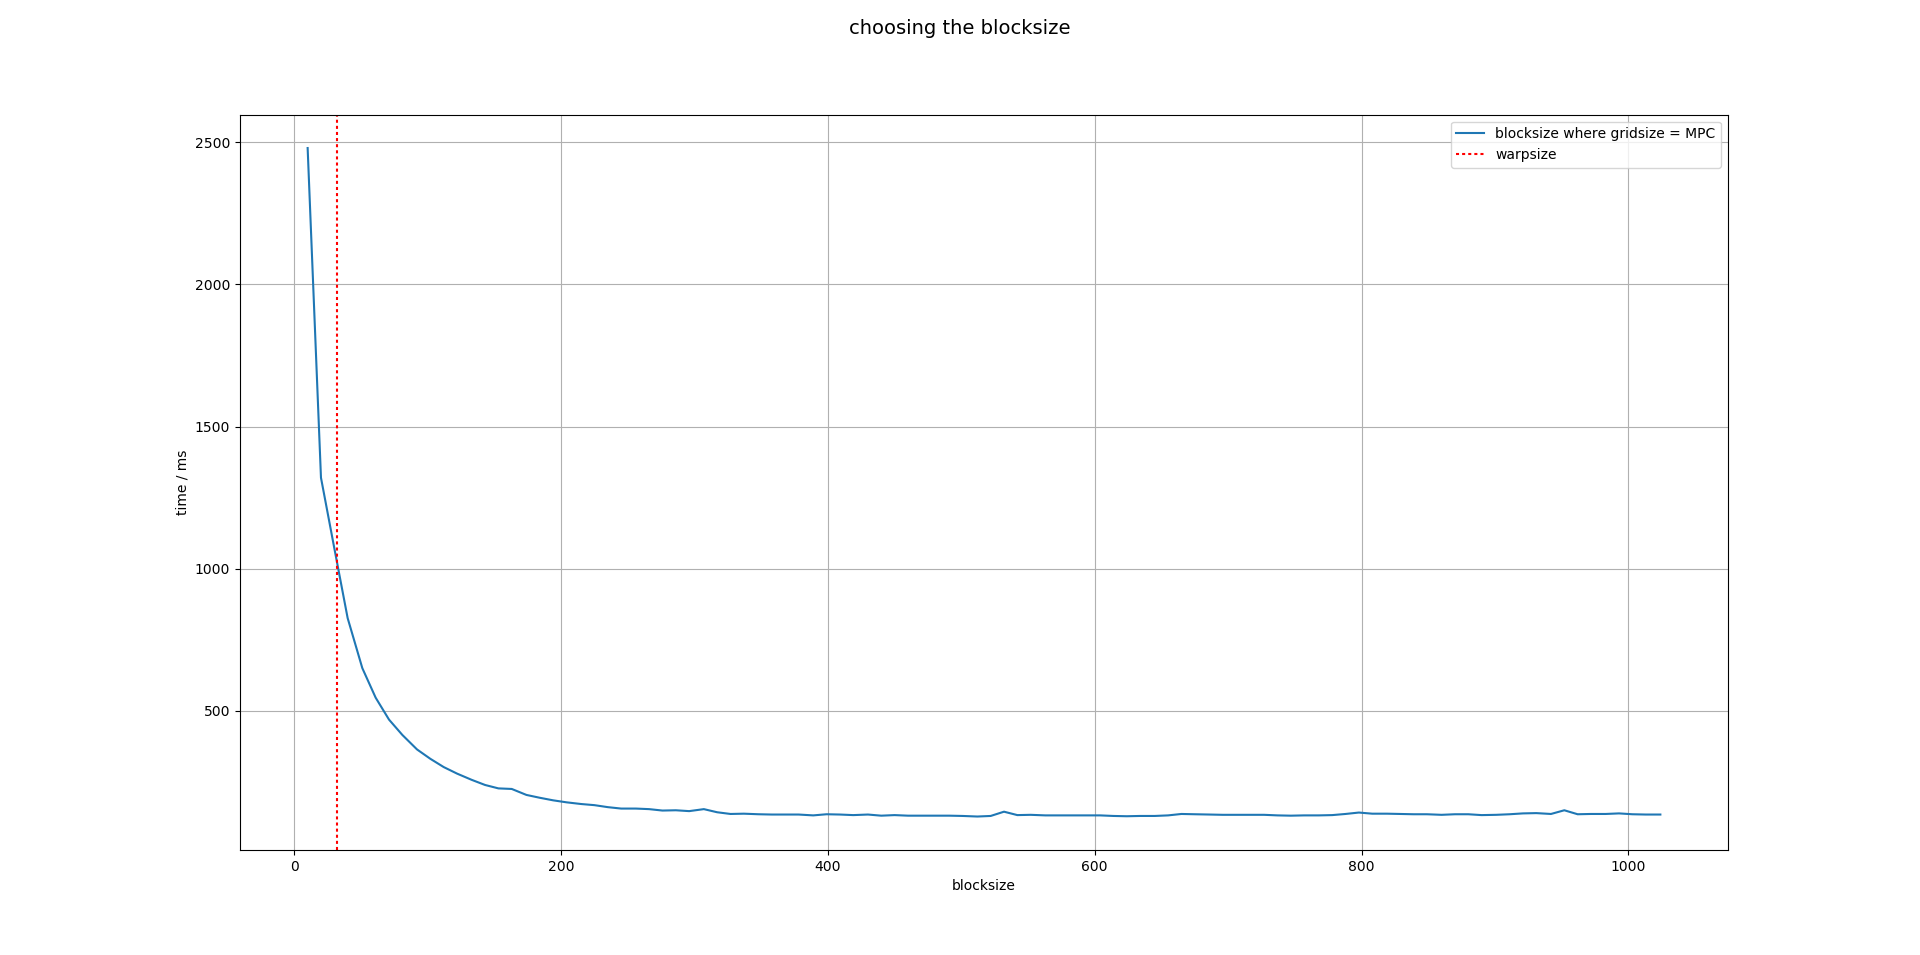
\includegraphics[width=\paperwidth]{img/blocksize.png}}
\end{frame}
\setbeamertemplate{navigation symbols}{}
\begin{frame}[plain]
	\makebox[\linewidth]{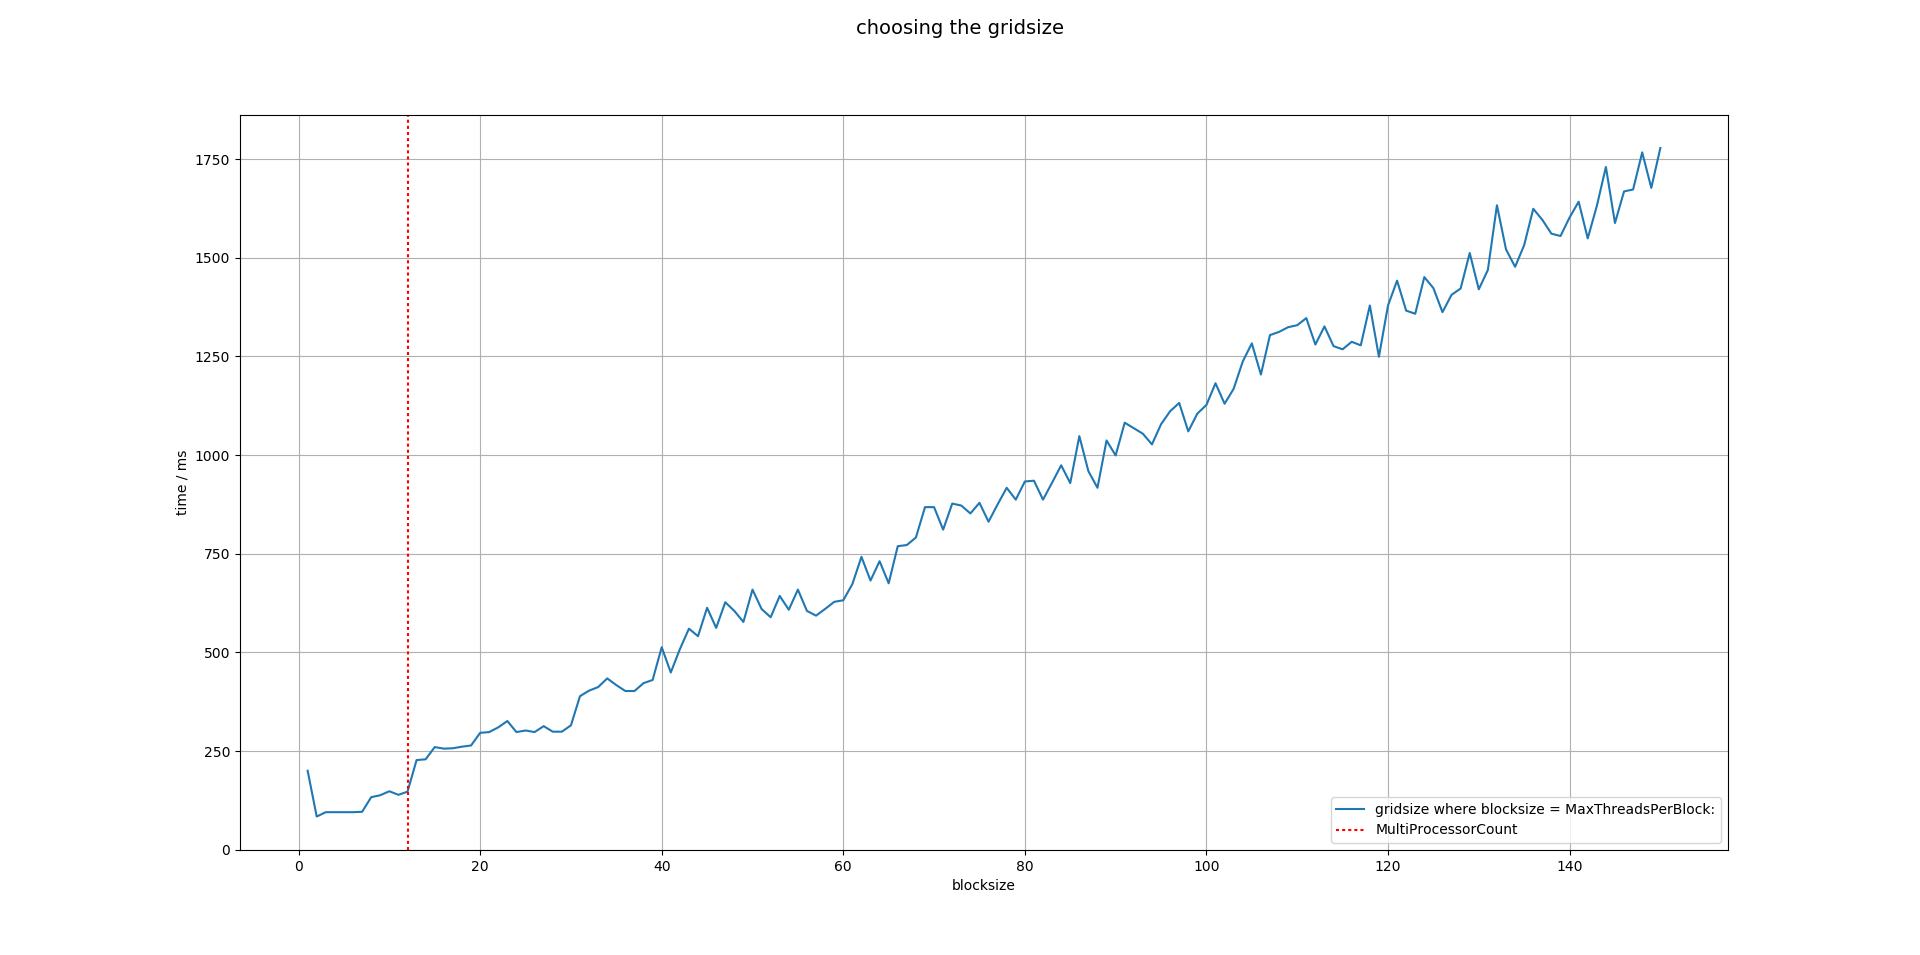
\includegraphics[width=\paperwidth]{img/gridsize.png}}
\end{frame}
\begin{frame}[plain]
	\makebox[\linewidth]{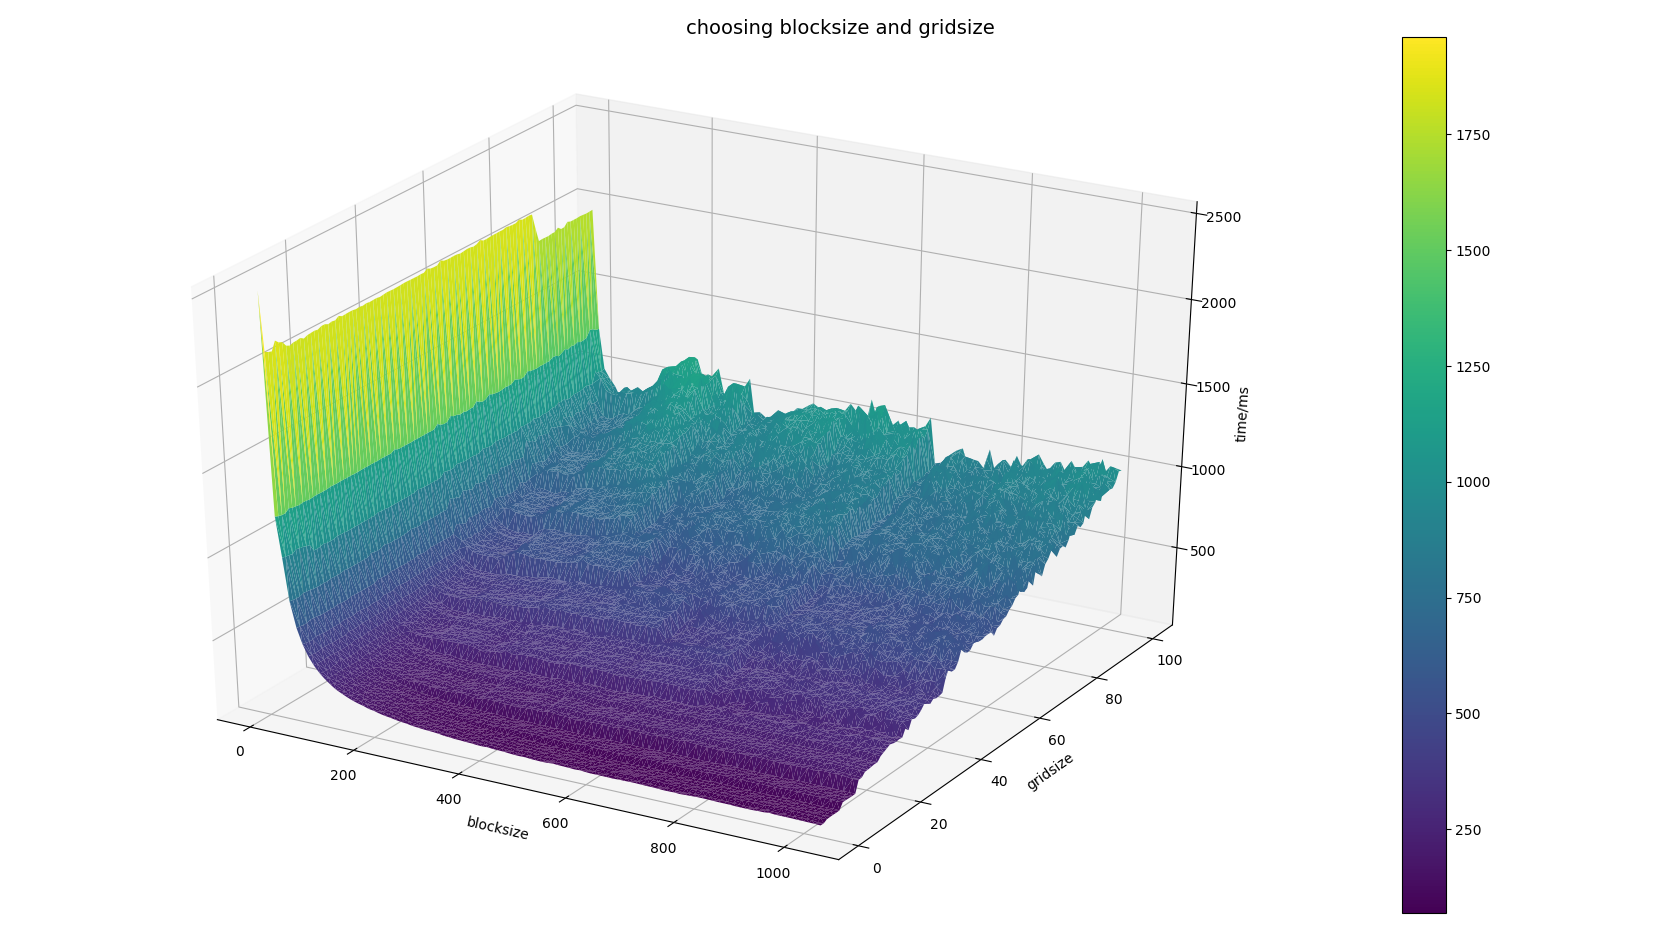
\includegraphics[width=\paperwidth]{img/block_grid_3d.png}}
\end{frame}
	\section{Solve - The modulus iteration algorithm} \label{sec_solve}
The last function, that had to be implemented was a solver for a PL function in abs-normal form. Given:
\begin{flalign*}
	a,b,Z,L,J,Y,m,n,\Delta y
\end{flalign*}
We want to calculate:
\begin{flalign*}
	\Delta x, \Delta z
\end{flalign*}

\subsection{Deducing a solution}
In \cite{Griewank2017} Multiple solutions with different properties in convergence and complexity have been suggested. Here we focus on the algorithm that in \cite{Griewank2017} is called modulus iteration algorithm. \\
For deducing this algorithm we first and foremost assume:
\begin{flalign*}
	\Delta y = 0
\end{flalign*}
It this is not the case, we can replace $b$ with $b'$:
\begin{flalign*}
	b' = b - \Delta y
\end{flalign*}
and replace $\Delta y$ with the zero-vector $O_m$. Now we can rearrange the equation system:
\begin{flalign*}
	\Delta y &= b + J \Delta x + Y |\Delta z| \\
	0 &= b + J \Delta x + Y |\Delta z| \\
	- b - Y |\Delta z| &= J \Delta x \\
	b + Y |\Delta z| &= J \Delta x (-1) \\
	J^{-1}(b + Y |\Delta z|) &= - \Delta x
\end{flalign*}
and obtain:
\begin{flalign}
	\Delta x = - J^{-1}(b + Y |\Delta z|) \label{eq_modulus_dx}
\end{flalign}
For calculating $\Delta z$ we can now use (\ref{eq_modulus_dx}):
\begin{flalign*}
	\Delta z &= a + Z \Delta x + L |\Delta z| \\
	&= a + Z \Big( - J^{-1}(b + Y |\Delta z|) \Big) +  L |\Delta z| \\
	&= a + Z \Big( -J^{-1}b - J^{-1}Y|\Delta z| \Big) +  L |\Delta z| \\
	&= a - ZJ^{-1}b - Z J^{-1}Y|\Delta z| +  L |\Delta z| \\
	&= a - ZJ^{-1}b - (Z J^{-1}Y - L)|\Delta z| \\
\end{flalign*}
Summarized:
\begin{flalign}
\Delta z &= c + S|\Delta z| \label{eq_modulus} \\
c		 &= a - ZJ^{-1}b \label{eq_c} \\
S		 &= L - Z J^{-1}Y \label{eq_S}
\end{flalign}

We can use this result to construct a fix-point iteration algorithm where we recalculate $\Delta z$ in each step until convergence. In the following we focus onto the implementation of this algorithm.

\subsection{Implementation}
Implementing this algorithms means calculating (\ref{eq_c}) and (\ref{eq_S}) once and using these to repeatedly calculate (\ref{eq_modulus}).
The key problem here is the calculation of $J^{-1}$, since this is the most expensive Operation. We decided to do a QR-decomposition of $J = QR$ and solving the linear equation system instead of calculating $J^{-1}$ directly. E.g. calculating $c$ is done in the following way:

\begin{enumerate}
	\item $J = QR$
	\item Solve $b = QRx$
		\begin{flalign*}
			QR x &= b \\
			x    &= solve(Rx = Qb)
	\end{flalign*}
	\item Calculate $c$:
	\begin{flalign*}
		c = a - Zx
	\end{flalign*}
\end{enumerate}
The calculation of $S$ follows the same  pattern. After convergence $\Delta x$ can be calculated according to (\ref{eq_modulus_dx}).

\subsection{Performance Experiment}

We did an experiment to benchmark the performance of our implementation. Obviously this only made sense as long as the results were correct. To verify this, we preceded as follows:
\begin{enumerate}
	\item Randomly generate a function in abs-normal form: $a,b,Z,L,J,Y, \Delta x$ according to (\ref{absnf}).
	\item Evaluate given function to obtain: $\Delta y$ and $\Delta z$
	\item Solve the system for $\Delta x$ and $\Delta z$ with the results of the previous step
	\item Verify if the resulting $\Delta x$ and $\Delta z$ match the original ones.
\end{enumerate}

We measured the runtime of the solve function in given context. To make sure, that each device works with the same data, we fixed the seed for the pseudo-random number generator. The results of this experiment can be found in fig \ref{fig_modulus_runtime}. 

\begin{figure}[ht]
	\centering
	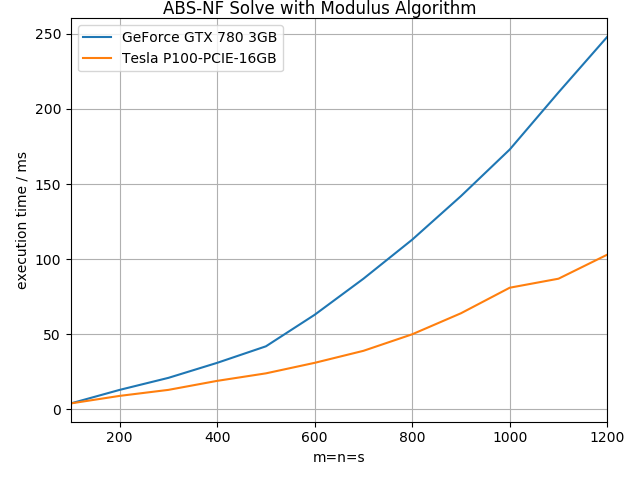
\includegraphics[width=0.6\textwidth]{img/solve_modulus.png}
	\caption{Runtime of the modulus solve implementation}
	\label{fig_modulus_runtime}
\end{figure}

\subsection{Analysis and Notes}
The implementation works correctly and the runtime results in fig. \ref{fig_modulus_runtime} behave as expected. We did not include the runtime of the serial version on purpose. This was for two reasons:
\begin{enumerate}
	\item The numpy implementation calculates the inverse of $J$ directly.
	\item We had to make sure, that each version operates on the exact same data, which we didn't
\end{enumerate}


	%------------------------------------------------------------------------
\begin{frame}
	\frametitle{Content}
	\framesubtitle{ABS-Normal Form}
	\begin{columns}[T] % align columns
		\begin{column}{.48\textwidth}
			
			\begin{center}
				{\Huge Final Thoughts}
			\end{center}
			
		\end{column}%
		\hfill%
		\begin{column}{.48\textwidth}
			\color{blue}\rule{\linewidth}{4pt}
			
			\setbeamertemplate{enumerate items}[default]
			\begin{enumerate}
				\item Einführung
				\item Aufgaben
				\item Evaluate
				\item Gradient
				\item Blocksize und Gridsize
				\item Solve
				\item \textbf{Final Thoughts}
			\end{enumerate}
		\end{column}%
	\end{columns}
\end{frame}
%------------------------------------------------------------------------
\begin{frame}[fragile]
	\frametitle{Final Thoughts}
	\framesubtitle{Was ist da?}
Was ist da nach der ersten Implementation?
\pause
\begin{lstlisting}
-------------------------------------------------------------------------------
Language                     files          blank        comment           code
-------------------------------------------------------------------------------
Python                          25            285            486           7451
C/C++ Header                     5             82            209           1256
C++                              7             41             19            334
-------------------------------------------------------------------------------
SUM:                            37            408            714           9041
-------------------------------------------------------------------------------
\end{lstlisting}
\pause
Dabei:
\begin{itemize}
	\item Working prototype in CUDA C++ und Python
	\item Unittests
	\item Coole Plot Generatoren
\end{itemize}
\end{frame}
%------------------------------------------------------------------------
\begin{frame}
	\frametitle{Final Thoughts}
	\framesubtitle{Was fehlt?}
	Was fehlt:
	\begin{itemize}
		\item <2-> Refactoring
		\item <3-> Funktionierende Implementierung des Gen. Newton solvers
		\item <4->Useability
		\item <5-> Anwendung
		\item <6->Numerische Checks der Ergebnisse bei größeren Daten
		\item <7-> Speichermanager
		\item <8-> Spezielle Wahl für Gridsize und Blocksize
		\item <9-> Multidevice Support
		\item <10-> Sparsity
		\item <11-> Math Tuning
	\end{itemize}
\end{frame}
%------------------------------------------------------------------------
\begin{frame}
	\frametitle{Quellen}
	\framesubtitle{ect.}
	\begin{itemize}
		\item Archiv Torsten Bosse
		\item Linear Algebra and its Applications - Griewank
		\item Cuda DOC
		\item $https://castingoutnines.wordpress.com/2010/01/12/piecewise-linear-calculus-part-2-getting-to-smoothness/$
	\end{itemize}
	
\end{frame}
%------------------------------------------------------------------------
\begin{frame}
	\frametitle{Quellen}
	\framesubtitle{Fixpunktiteration}
	\begin{center}
		\animategraphics[height=6cm, width=10cm,controls]{1}{img/n/n}{0}{4}
	\end{center}
\end{frame}
\end{document}